\documentclass[a4paper,11pt]{memoir}
\usepackage{mathtools}
\usepackage{graphicx}
\usepackage[utf8]{inputenc}
\usepackage{float}
\begin{document}
\chapter{Spørgsmål til vejleder mht. draft kredsløb i programmet Plecs}

\newpage

\begin{figure}[htbp]
\centering
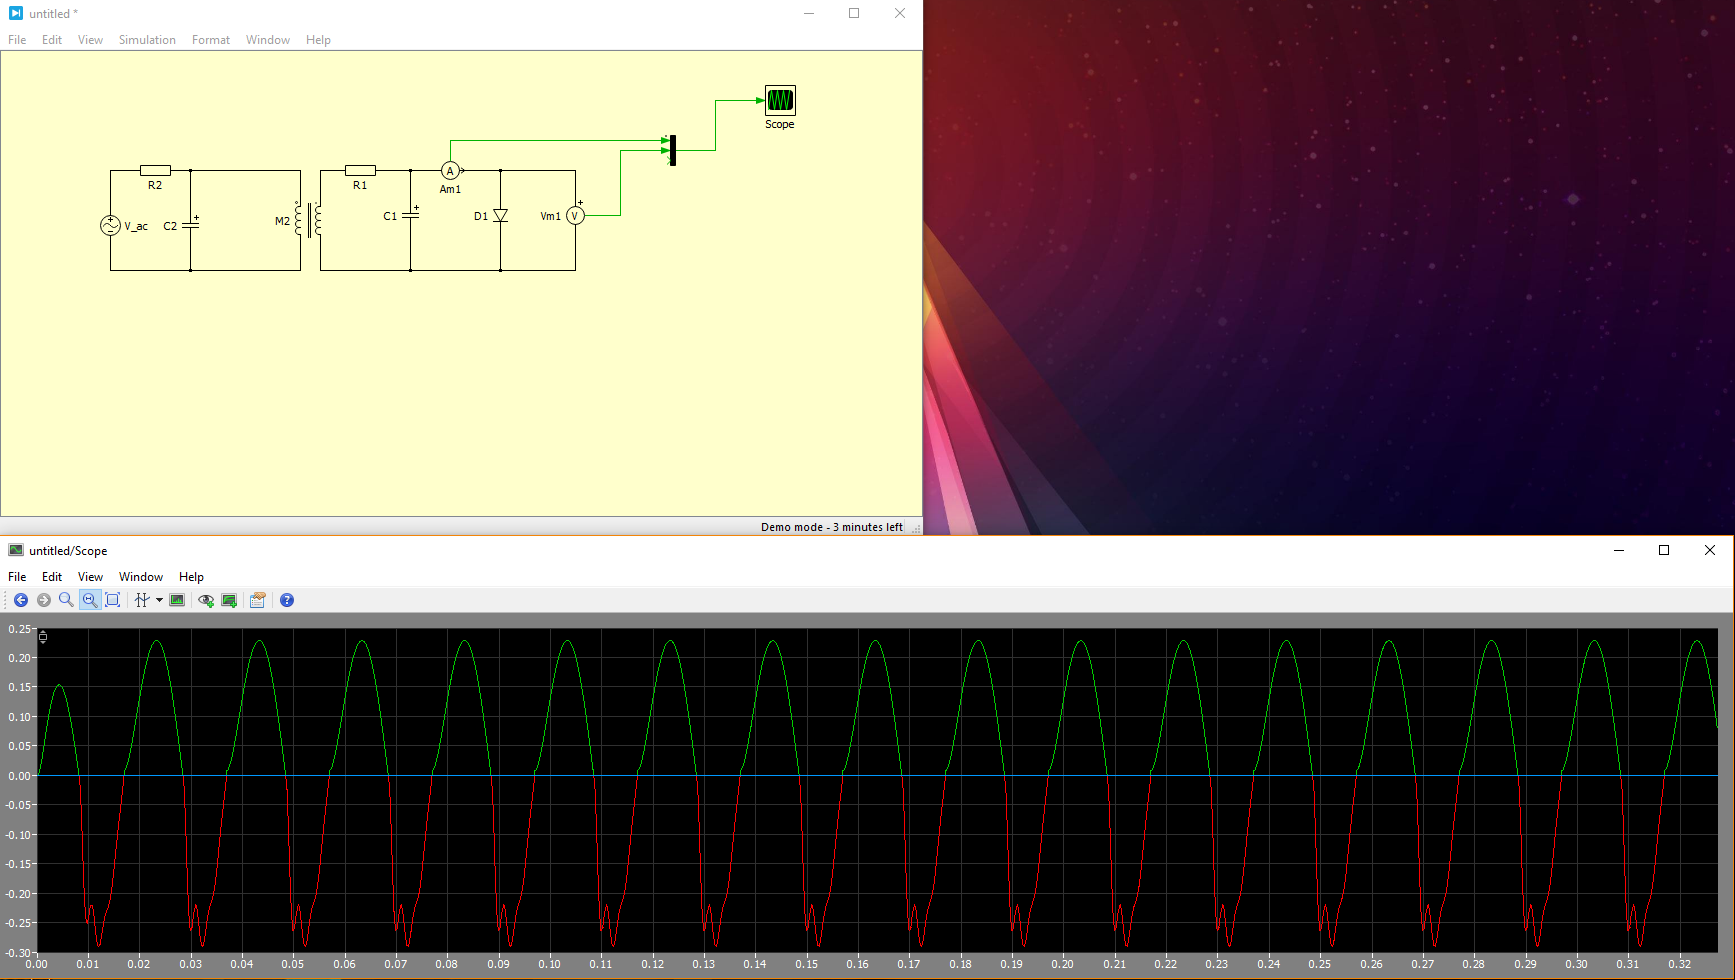
\includegraphics[width=13cm]{Schematics/161031_Plecs1.png}
\caption{Opstilling1: venstrerettet transformer}
\end{figure}

\begin{figure}[H]
\centering
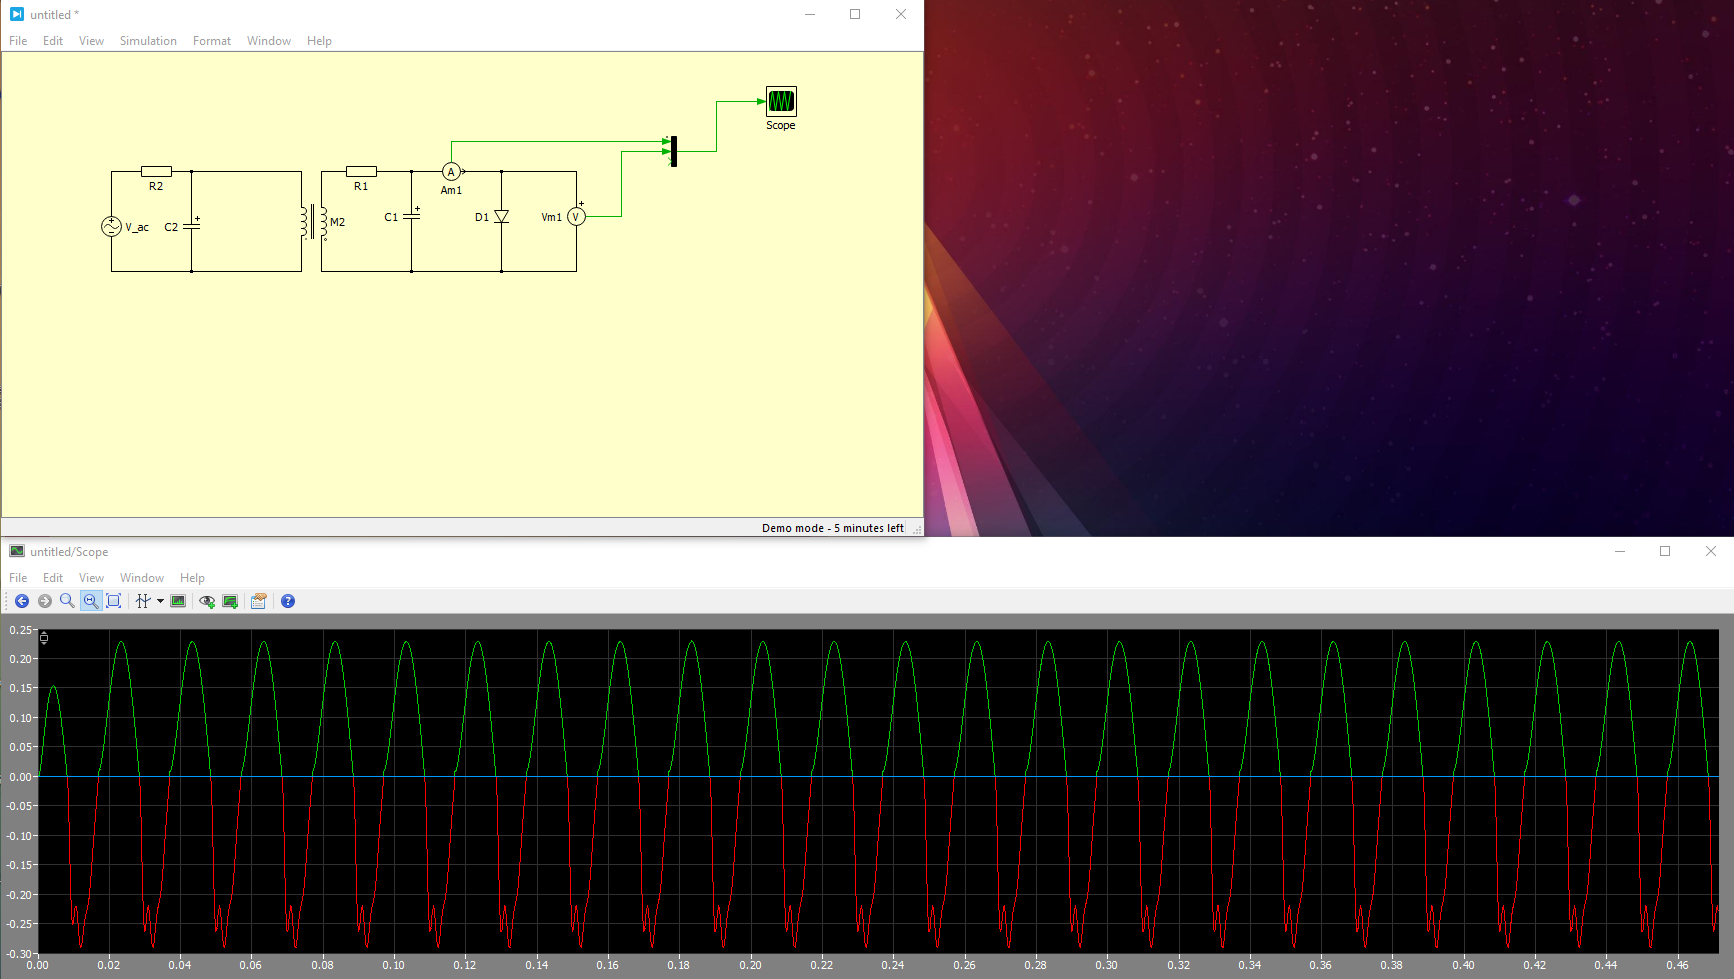
\includegraphics[width=1\textwidth]{Schematics/161031_Plecs2.png}
\caption{Opstilling2: højrerettet transformer}
\end{figure}
\newpage

Herover er der to billeder med diagrammer og simulationer fra det samme kredsløb, med den eneste forskel af at transformeren i midten er spejlet. Dette er gjort som forsøg, for at test som dette ville gøre nogen forskel.

Transformeren i midten skulle forhåbentligt repræsentere den trådløse energioverførsel.

Opstillingen er i alt sin simpelhed opbygget således, fra venstre mod højre:

\begin{itemize}
\item En strøm kilde der leverer AC strøm, sinus-oscillerende
\item R2+R1: Resistore
\item C2+C1: Kapacitatore
\item M2: transformer
\item Amperemeter
\item D1: Diode
\item Voltmeter
\end{itemize}

Alle Enhedernes værdier er Plecs' valgte standart værdier. Der er ikke foretaget nogle ændringer i dem.

Ideen med opstillingen er, at den skulle på den simpleste mulige måde, repræsentere trådløs energioverførsel over to spoler. Dette skulle så kunne simuleres, derfor er dioden med, så der er noget at måle på. I dette tilfælde er der bare sat et voltmeter hen over, og et amperemeter til.

De to spoler skulle repræsenteres af transformeren. Vi er ikke helt sikre på om dette er på nogen måde korrekt. Dette er kun antaget ud fra andre skemaer, som har benyttet samme symbol som transformeren.

\section{Spørgsmål}
\begin{enumerate}
\item Er den overordnede ide mht. at sende strøm hen over transformeren, for at simulere to spoler, med et felt i mellem til at overføre energi, der kan måles hen over dioden?
\item Hvor går vi herfra mht. modellering af diagrammer?
\item Hvilke data, ville give de mest "realistiske" tests?
\item Hvilke tests ville give mening at udføre for at måle effektiviteten af opstillingen? Både i programmet og laboratorie.
\item Har du mulighed for at give os en nøgle til programmet Plecs, eller sende os videre hos AAU til en der kan? Det er umådeligt simpelt at arbejde med og vi kunne godt tænke os at udforske dets potentiale. Vi vil have mulighed for at spørge 2 semesters studerende og frem om hjælp. Programmet bruges af energistuderende allerede fra 2. semester.
\end{enumerate}
Eventuelle kommentarer til modelleringsdelen af projektet er meget velkommende.

Ps.ja, dokumentet er skrevet i latex af ren og skær indøvelse og rutine dannelse.
\end{document}